\documentclass[12pt,oneside,openany,a4paper]{book} % This style for A4 format.

\input{./AuxFiles/Packages}

%%%%%%%%%%%%%%%%%%%%%%%%%%%%%%%%%%%%%%%%%%%%%%%%%%%%%%%%%%%%%%%%
%% Document settings
\title{Mitigating Logistics Friction in Global Chokepoints: An Agentic AI Framework for Indian Export-Import Resilience}
\subCode{AI481P}
% Note: While using the template for IDP, the \Department cmd is not used (discarded automatically) in IDP. The Certificate page uses \guideDeptA[]{} cmd in IDP.
\Department[AIML]{Artificial Intelligence and Machine Learning}
\academicYear{2025-26}

%%%%%%%%%%%%%%%%%%%%%%%%%%%%%%%%%%%%%%%%%%%%%%%%%%%%%%%%%%%%%%%%
%% Report Type:
%%%%%%%%%%%%%%%%%% For Plagiarism Check %%%%%%%%%%%%%%%%%%%%%%%
%% Uncomment \EnPlagReport line, before plagiarism check to remove Certificate, Declaration, Acknowledgement and TOC pages.
%\EnPlagReport

%%%%%%%%%%%%%%%%%%%%%% DTL report %%%%%%%%%%%%%%%%%%%%%%%%%%%%%
%% Uncomment \DTLProject line, if the report is for DTL project.
%\DTLProject

%%%%%%%%%%%%%%%%%%%%%% IDP report %%%%%%%%%%%%%%%%%%%%%%%%%%%%%
%% Uncomment \IDPProject line, if the report is for IDP project.
%\IDPProject

%%%%%%%%%%%%%%%%%%%%% Internship report %%%%%%%%%%%%%%%%%%%%%%%
%% Uncomment \InternProject line, if the report is for Minor project.
%%\InternProject

%%%%%%%%%%%%%%% Minor (or) Major report %%%%%%%%%%%%%%%
%% Uncomment \MinorProject line, if the report is for Minor project.
\MajorProject

%%%%%%%%%%%%%%%%%%% For PG program %%%%%%%%%%%%%%%%%%%
%% Uncomment \pgProgram command and define appropriate values for \MastersIn{} and \pgProgramName{}

%\pgProgram%
%\MastersIn[B.E]{Bachelor of Engineering}
%\pgProgramName{Artificial Intelligence and Machine Learning}

%%%%%%%%%%%%%%%%%%%%%%%%%%%%%%%%%%%%%%%%%%%%%%%%%%%%%%%%%%%%%%%%
%% Student Details%%%
\stuNameA{Ananth M Athreya}
\stuUSNA{1RV22AI007}
\stuNameB{Anant Tewari}
\stuUSNB{1RV22CD005}
\stuNameC{Kiran Aithal}
\stuUSNC{1RV22CD022}
\stuNameD{Pranav S K}
\stuUSND{1RV22CD041}
%\stuNameE{Advaith Singh}
%\stuUSNE{1RV22CS012}
%\stuNameF{Arjith Sinha}
%\stuUSNF{1RV22IM013}

%%%%%%%%%%%%%%%%%%%%%%%%%%%%%%%%%%%%%%%%%%%%%%%%%%%%%%%%%%%%%%%%
%% Guide Related commands
%% Internal Guide %%
% Have to give both short form and long of Department Name
\guideNameA{Dr. B Sathish Babu}
\guideDesignationA{Professor and Head}
\guideDeptA[AIML]{Artificial Intelligence and Machine Learning}
\guideOrgA{RV College of Engineering}

%% External Guides (Don't Use for Internship; U have '\projectCoOrdNameA{}' for Internship) %%
%\guideNameB{Dr. Ramavenkateshwaran}
%\guideDesignationB{Assistant Professor}
%guideDeptB{Dept. of ECE}
%\guideOrgB{RV College of Engineering}

%\guideNameC{Dr. Ramavenkateshwaran}
%\guideDesignationC{Assistant Professor}
%\guideDeptC{Dept. of ECE}
%\guideOrgC{RV College of Engineering}

%%%%%%%%%%%%%%%%%%%%%%%%%%%%%%%%%%%%%%%%%%%%%%%%%%%%%%%%%%%%%%%%
%% Esteem members related commands
%% Pannel Members %%
\panelMemberNameA{Dr. B Sathish Babu}
\panelMemberDesigA{Professor and Head}
\panelMemberDeptA[AIML]{Artificial Intelligence and Machine Learning}
\panelMemberNameB{Mr. Rushikesh Anil Padaki}
\panelMemberDesigB{Assistant Professor}
\panelMemberDeptB[AIML]{Artificial Intelligence and Machine Learning}

% Added Ver 3.6 & 3.9
%% Project co-ordinators (for Internal RVCE) & Internship co-ordinators (for COE as well as Internship company Manager or Supervisor)
\projectCoOrdNameA{Mr. Rushikesh Anil Padaki}
\projectCoOrdDesigA{Assistant Professor}
\projectCoOrdDeptA[AIML]{Artificial Intelligence and Machine Learning}
% Not used for IDP and Internship
\projectCoOrdNameB{Mrs. Harshitha V}
\projectCoOrdDesigB{Assistant Professor}
\projectCoOrdDeptB[AIML]{Artificial Intelligence and Machine Learning}
%\projectCoOrdNameC{Prof. Subramanya K N}
%\projectCoOrdDesigC{Assistant Professor}

% Added Ver 3.9
%% Departmental Internship co-ordinator details (internal to RVCE)
\internCoOrdNameA{Prof. P Narashimaraja}
\internCoOrdDesigA{Assistant Professor}
\internCoOrdDeptA[ECE]{Electronics and Communication Engineering}

%%%%%%%%%%%%%%%%% Esteemed Members %%%%%%%%%%%%%%%%%%
\HOD{Dr. Shantha Rangaswamy}
\Principal{Dr. K. N. Subramanya}
% For IDP only
\DeanAcademics{Dr. M.V. Renukadevi}
\VicePrincipal{Dr. Geetha K S}
%%%%%%%%%%%%%%%%%%%%%%%%%%%%%%%%%%%%%%%%%%%%%%%%%%%%%%%%%%%%%%%%
%%%%%%%%%%%%%%%%%%%%%  QRL %%%%%%%%%%%%%%%%%%%%%%%%%%
\QRurl{https://drive.google.com/drive/folders/1Oa2priCm6g9bSkNLgT98ikuE1_H7rI6Z?usp=sharing}
%\QRurl{https://drive.google.com/open?id=1jm-POmuq-ZZ1tT5m-xAdCDRnwvLZH8q-}

%%%%%%%%%%%%%%%%%%Draft report%%%%%%%%%%%%%%%%%%
%\DraftCopy %Not yet implemented, if anyone interested, do contact me at pnarashimaraja@rvce.edu.in (or) narashimaraja@gmail.com
%%%%%%%%%%%%%%%%%%%%%%%%%%%%%%%%%%%%%%%%%%%%%%

%%%%%%%%%%%%%%%%%% Glossaries & Acronyms %%%%%%%%%%%%%%%%%%
\newglossary[sym]{symbolList}{sym1}{sym2}{List of Symbols}
\makeglossaries
% Acronyms
\loadglsentries{./AuxFiles/Glossaries}
\renewcommand{\glspostdescription}{}% To remove dot at the end
%%%%%%%%%%%%%%%%%%%%%%%%%%%%%%%%%%%%%%%%%%%%%%

%%%%%%%%%%%%%%%% Bibliography %%%%%%%%%%%%%%%%%%%%%
\usepackage[backend=bibtex,style=ieee,sorting=none]{biblatex}
% If backend is set to bibtex, then configure texmaker Bi(La)Tex with "bibtex %", 
% however biber is recommended for sorting=none to work correctly.
\addbibresource{./AuxFiles/ProjectBib.bib}%Add bib file with extention
%%%%%%%%%%%%%%%%%%%%%%%%%%%%%%%%%%%%%%%%%%%%%%

%%%%%%%%%%%%%%%%WaterMark%%%%%%%%%%%%%%%%%%%%%
%% Use it only after Biblatex
%% Uncomment the following lines for watermarking and run it more than 2 times for proper alignment
\usepackage{background}
\backgroundsetup{scale=1, angle=0, firstpage = true, opacity=0.5, contents={
\begin{tikzpicture}[remember picture, overlay]
\node at ([yshift=0pt, xshift=0pt]current page.center){\includegraphics[width=0.6\textwidth]{Figures/RVlogoVecW}};
\end{tikzpicture}
}}

\begin{document}
\NoBgThispage% Don't remove this command, even if you want logo on the first page.	
\maketitle
\StuNameBUsedfalse
\StuNameCUsedfalse
\StuNameDUsedfalse
%\pagestyle{empty}
\newpage
\ifDrf
% Remove Certificate, Declaration, Acknowledgement and TOC
\else
\begin{spacing}{1.5}
\input{./CoverPages/Certificate}
\ifINT
\else
\newpage
\input{./CoverPages/Declaration}
\fi
\newpage
\ifINT
\input{./CoverPages/Ack_int}
\else
\input{./CoverPages/Ack}
\fi
\newpage
\pagenumbering{roman}
\ifINT
\chapter*{Executive Summary}
\input{./CoverPages/Summarys}
\else
\chapter*{Abstract}
\input{./CoverPages/Abstract}
\fi

\end{spacing}
\newpage
\pagestyle{fplain}
\begin{spacing}{1.5}
	\tableofcontents	
\end{spacing}
\newpage
\begin{spacing}{1.5}
	\cleardoublepage
	\addcontentsline{toc}{chapter}{\listfigurename}
	\listoffigures	
\end{spacing}
\newpage
\begin{spacing}{1.5}
	\cleardoublepage
	\addcontentsline{toc}{chapter}{\listtablename}
	\listoftables	
\end{spacing}
\newpage
\printglossary[type=\acronymtype, title= Abbreviations, toctitle=Abbreviations]
\newpage
\printglossary[type=symbolList, title= List of Symbols, toctitle=List of Symbols]
\fi
\mainmatter
\onehalfspacing
\pagestyle{mplain}
\glsresetall

%Chapter 1 
\ifINT
\input{./Chapter1/chapter1-Profile}
\else
\chapter{Introduction}
This chapter provides a comprehensive introduction to the proposed project. It explains the
background of the problem domain, significance of the work, objectives, scope, and
methodology adopted for the project. The chapter also presents a review of existing literature,
identifies research gaps, and outlines the overall organization of the report. The purpose of
this chapter is to provide readers with a clear understanding of the motivation, need, and
approach of the proposed work.

\section[Introduction]{\textbf{Introduction}}
Global trade is increasingly defined by Logistics Friction a composite of temporal, financial, and physical delays at critical maritime chokepoints. Specifically in consideration of ongoing events we can consider the supply and logistics of Crude Oil, LNG and other petroleum products and by products which have been shown to be vulnerable. 

Large-scale enterprises employ sophisticated risk-modeling, Indian SMEs remain vulnerable to the "bullwhip effect" caused by sudden shifts in transit verification, insurance spikes, and port congestion. 

The Bullwhip Effect is a supply chain phenomenon where small fluctuations in consumer demand at the retail level cause progressively larger fluctuations at the wholesale, distributor, and manufacturer levels.


\subsection[Terminology and Definitions]{\textbf{Terminology and Definitions}}

This section defines the key technical terms, abbreviations, and domain-specific concepts used throughout this report.
\begin{table}[H]
\centering
\resizebox{\textwidth}{!}{
\begin{tabular}{|p{4cm}|p{11cm}|}
\hline
\textbf{Term} & \textbf{Definition} \\
\hline
\textbf{Shock Location / Disruption Node} & A specific geographical point or transit corridor (e.g., chokepoint, port, road link) experiencing supply chain friction, congestion, or security threats. \\
\hline
\textbf{Signal Type} & The classification of the disruption or external risk factor triggering a supply-chain alert. \\
\hline
\textbf{Severity Multiplier} & A coefficient that scales baseline time and cost variables to simulate the intensity of a disruption.\\
\hline
\textbf{Strategic Preference} & The trade-off priority chosen by a logistics manager (or agent) to optimize the supply network. \\
\hline
\textbf{Landed Cost} & The total cumulative cost of buying, transporting, insuring, and storing inventory until it reaches its final destination market. \\
\hline
\textbf{Transit Days} & The lead time (in days) required for cargo to travel along the chosen path from the supplier to the destination market. \\
\hline
\textbf{Response Latency} &  The decision-making time elapsed between detecting a supply chain shock and implementing a mitigation strategy (such as rerouting or restocking). \\
\hline
\textbf{TEU (Twenty-foot Equivalent Unit)} & A standardized unit of measurement for container capacity in maritime shipping, equivalent to one 20-foot container. Used to measure vessel capacity and cargo volume. \\
\hline
\textbf{Bunker Cost} & The cost of marine fuel (bunker oil) required to power a vessel during transit. Bunker costs fluctuate based on global oil prices and significantly impact overall shipping expenses. \\
\hline
\end{tabular}
}
\caption{Terminology and Definitions}
\label{tab:terminology}
\end{table}

\section[Overview of the Project Topic]{\textbf{Overview of the Project Topic}}

The domain of this project resides at the intersection of Agentic Artificial Intelligence and Maritime Logistics, a sector critical to global trade. In modern systems, the ability to automate complex decision-making through autonomous agents has become a cornerstone of supply chain resilience. Recent advancements in Large Language Models (LLMs) and multi-agent systems have moved the field beyond static predictive models toward dynamic, goal-oriented frameworks capable of independent reasoning. This evolution holds immense academic and industrial relevance, as it addresses the persistent challenge of "logistics friction" within highly volatile maritime chokepoints. By integrating real-time data ingestion with agent-driven optimization, the technology plays a vital role in mitigating the bullwhip effect and reducing transit uncertainties. For Indian enterprises, particularly SMEs, this framework offers a robust mechanism for maintaining export-import competitiveness, transforming reactive crisis management into proactive, intelligent resilience against global trade shocks.

\subsection[Global Scenario]{\textbf{Global Scenario}}

Technological developments in global trade are increasingly pivoting toward AI-driven resilience. Organizations like the World Trade Organization (WTO) and major shipping conglomerates are prioritizing "Logistics Friction" mitigation to stabilize global maritime trade. Recent innovations include predictive risk-modeling and decentralized logistics, yet the worldwide demand for autonomous execution remains high. Global supply chains, particularly those passing through maritime chokepoints like the Red Sea or the Suez Canal, face escalating vulnerabilities to geopolitical and administrative shocks. While advanced economies are integrating multi-agent systems to handle these disruptions, a significant technological gap persists in transit corridors affecting developing markets. The maritime industry is currently shifting from simple problem detection to agent-driven real-time optimization, with international research trends focusing on goal-oriented autonomous frameworks. This global demand highlights the project's significance in creating scalable, intelligent solutions for international trade stability.

\subsection[Societal Relevance]{\textbf{Societal Relevance}}

This project carries significant societal relevance by safeguarding the livelihoods dependent on India's export-import (EXIM) sector. Small and Medium Enterprises (SMEs) form the backbone of the Indian economy, yet they are disproportionately impacted by the "bullwhip effect" when maritime disruptions occur. By providing these enterprises with accessible, agentic AI tools, the project promotes economic equity and industrial sustainability. It transforms complex, manual logistics processes into automated, efficient workflows, reducing the financial strain caused by sudden insurance spikes or port congestion. Furthermore, the framework supports national economic resilience by ensuring the steady flow of essential commodities like crude oil and LNG. Societally, this leads to price stabilization and increased security within manufacturing and trading communities, contributing to a more robust national economy through the technological empowerment of smaller industrial players.

\subsection[Problem Area]{\textbf{Problem Area}}

The core problem area is the critical gap between "Detection" and "Autonomous Execution" in current logistics management. Existing maritime systems are predominantly reactive and manual, leaving Indian SMEs vulnerable to rapid disruptions at maritime chokepoints. When a transit delay occurs, these organizations often lack the data-infrastructure and risk-modeling capabilities required to implement proactive mitigation. Furthermore, most modern AI solutions are designed for data-rich environments, creating a "Data-Infrastructure Gap" for SMEs operating in data-sparse, developing-economy contexts. If unaddressed, minor transit delays escalate into severe domestic supply chain failures and unmanageable landed costs. This problem requires immediate attention because traditional manual intervention is insufficient to manage the cascading effects of modern geopolitical shocks, necessitating an intelligent framework capable of independent reasoning and rapid response to mitigate Logistics Friction.

\section[Specific Details of the Project Topic]{\textbf{Specific Details of the Project Topic}}

This section provides a detailed technical breakdown of the proposed Agentic AI framework, encompassing the core concepts, technological stack, and architectural design principles.

\subsection{Technical Concepts}
The project integrates several advanced domains to create a robust supply-chain solution:
\begin{itemize}
    \item \textbf{Digital Twin:} A virtual, real-time representation of the physical supply-chain network—covering suppliers, ports, chokepoints, and warehouses—used to simulate shocks and test responses.
    \item \textbf{Agentic Orchestration:} Multi-agent workflows where specialized LLM-based autonomous agents collaborate via role-playing and prompt chaining to solve complex routing problems.
    \item \textbf{Graph Theory \& Network Optimization:} Modelling logistics lanes as directed graphs and using \textbf{Dijkstra's Algorithm} to calculate optimal paths based on dynamic weights like transit days and landed costs.
    \item \textbf{Stochastic Inventory Management:} Implementing the \textbf{Chopra Safety Stock Equation} to model lead-time variability and calculate buffer stocks required to avoid stockouts during shocks.
\end{itemize}

\subsection{Technologies, Tools, and Frameworks}
The implementation leverages a modern, high-performance stack:
\begin{itemize}
    \item \textbf{Backend:} Python (FastAPI) for high-performance REST APIs and asynchronous processing.
    \item \textbf{Orchestration Framework:} \textbf{CrewAI} for agent role definition and task delegation, powered by \textbf{Gemini-Flash} LLMs via the Google AI Studio API.
    \item \textbf{Graph Modeling:} The \texttt{networkx} library for building and managing the directed graph of the global logistics network.
    \item \textbf{Frontend:} React (Vite) for a glassmorphism dashboard, using \textbf{Leaflet} (\texttt{react-leaflet}) for interactive, geospatial visualization of routing paths.
\end{itemize}

\subsection{System Architecture and Working Principle}
The system operates as a reactive closed-loop pipeline where external shock events trigger a multi-stage response. First, the Friction Sentry maps unstructured signals to quantitative shock parameters. Second, the Agentic Optimizer uses specialized agents (Logistics Optimizer and Cost Analyst) to identify alternate routes and check inventory levels. Finally, the Communicator Agent compiles an actionable JSON payload to update the React frontend dashboard with optimized routing and financial metrics.

\subsection{Major Modules / Components}
The framework is divided into several specialized functional modules:
\begin{itemize}
    \item \textbf{Friction Sentry:} Receives raw event signals and translates them into structured risk variables such as insurance spikes and port congestions.
    \item \textbf{Execution \& Routing Engine:} Maintains the directed graph topology and runs network routing algorithms under both normal and shocked states.
    \item \textbf{Dynamic Inventory Manager:} Tracks stock levels, calculates daily demand depletion, and handles simulated emergency replenishment.
    \item \textbf{Agentic Solver (CrewAI):} The core intelligence unit comprising the Logistics Optimizer, Cost/Strategy Analyst, and SME Communicator agents.
    \item \textbf{Digital Twin UI:} An interactive geospatial React application showing baseline vs. optimized routes and financial/operational performance cards.
\end{itemize}

\subsection{Real-World Applications}
Practical applications include dynamic rerouting of cargo to avoid high-risk maritime zones (e.g., bypassing the Red Sea via the Cape of Good Hope) and port congestion mitigation by automatically switching destination ports (e.g., from Nhava Sheva to Mundra). Most importantly, it empowers Indian SMEs with automated inventory protection strategies that are typically only accessible to large multinational corporations.

\section[Purpose and Motivation]{\textbf{Purpose and Motivation}}

The primary purpose of this project is to bridge the critical gap between disruption detection and autonomous response in maritime logistics. As global trade becomes increasingly volatile, the practical need for a system that can not only predict shocks but also execute mitigation strategies independently has become paramount. This work is inspired by the necessity to protect vulnerable economic actors, such as Indian SMEs, from the cascading effects of geopolitical instability.

The motivation for this work stems from several fundamental challenges observed in existing systems:
\begin{enumerate}
    \item \textbf{Neglect of Upstream Maritime Shocks}: Existing predictive systems predominantly focus on downstream retail inventory and e-commerce environments, failing to account for critical upstream disruptions at maritime chokepoints like the Suez Canal or the Red Sea.
    \item \textbf{The Detection-to-Action Gap}: Current multi-agent frameworks excel at producing analytical reports from global signals but still require manual human execution to implement responses, leading to costly delays.
    \item \textbf{Reliance on Historical Data}: Modern replenishment models depend heavily on historical datasets, leaving them unable to simulate or mitigate unpredictable, real-time geopolitical transit shocks that have no historical precedent.
    \item \textbf{Underutilization of Agentic Tool Coordination}: While autonomous supply chain models exist, they often fail to leverage the full power of Agentic AI to coordinate diverse toolkits for the automated execution of complex user tasks, such as simultaneous rerouting and inventory restocking.
\end{enumerate}

By addressing these limitations, this project holds immense industrial and societal importance, transforming traditional reactive supply chain management into a proactive, agent-driven digital twin capable of ensuring global trade resilience.


\section[Problem statement]{\textbf{Problem statement}}
The project aims to develop a route-aware Agentic AI framework for Indian SMEs facing maritime shipping shocks. By transitioning from reactive manual management to autonomous execution, it mitigates "Logistics Friction" in data-scarce environments. This enhances EXIM resilience and prevents global bottlenecks from cascading into domestic failures.
\section[Objectives]{\textbf{Objectives}}
\begin{enumerate}
\item Design a Multi-Agent System (MAS) using LangChain/CrewAI to continuously ingest unstructured geopolitical signals and quantify them into measurable Logistics Friction variables within the Red Sea and Strait of Hormuz corridors.
\item Map a multi-tier logistics network using NetworkX to create a functional Digital Twin that visualizes and calculates how shipping shocks propagate from international maritime nodes to domestic Indian warehouses through Semantic Network queries.
\item Enable AI agents to move beyond analytical reporting by autonomously generating one-click actionable recommendations, including alternate maritime routing, dynamic buffer-stock adjustments, and backup supplier identification.
\item Establish a rigorous mathematical baseline to demonstrate significant cost reductions and drastically faster response times compared to traditional, manual SME planning processes.
\item Build a comprehensive Tableau Dashboard fed by the Digital Twin's output to provide SMEs with real-time "What-If" scenario simulations, cost-risk evaluations, and visual decision-support tools.
\end{enumerate}

\section[Scope and Relevance]{\textbf{Scope and Relevance}}

The scope of this project is concentrated on the development of an agentic digital twin for maritime logistics, specifically addressing upstream disruptions at global chokepoints. Included in this scope are real-time disruption parsing (Friction Sentry), autonomous multi-agent optimization using CrewAI, and geospatial visualization for Indian EXIM routes. The system incorporates dynamic inventory management using the Chopra equation and Dijkstra-based rerouting. However, the project excludes the orchestration of physical last-mile delivery fleets and does not integrate real-time satellite imagery for hardware-level port monitoring, relying instead on structured semantic signals.

The project holds high industrial relevance by offering SMEs technological tools previously reserved for multinational corporations, reducing the financial impact of the bullwhip effect. Academically, it contributes to the evolving field of agentic AI by demonstrating goal-oriented tool coordination for complex problem-solving. Societally, it fosters economic resilience through stabilized export-import flows, ensuring that vital supply chains remain operational despite geopolitical shocks.

\section[Literature Review]{\textbf{Literature Review}}
This section provides a detailed review of existing research, systems, technologies, and
methodologies related to the project domain.
\subsection[Literature Survey]{\textbf{Literature Survey}}
Recent work on agentic AI has shifted the discussion in supply chain management from passive prediction to autonomous execution. Early examples focus on real-time inventory management using distributed cloud architectures and machine learning, showing how agentic systems can combine forecasting with action in operational settings \cite{Tiwari2025}. In retail, agentic AI has been positioned as a mechanism for predictive analytics, autonomous customer interaction, and supply chain automation, especially where responsiveness and personalization are essential \cite{Kalisetty2024,KalisettySingireddy2023}. Extending beyond retail, agentic decision-making has also been proposed for food supply chains, where autonomy is framed as a way to improve control in complex and time-sensitive environments \cite{Pamisetty2024}.  

A recurring constraint in these applications is data sparsity, particularly for SMEs. Lightweight neural architectures have therefore been proposed for demand forecasting in low-data environments \cite{GuptaMehta2024}, while federated learning has been suggested as a privacy-preserving method for collaborative inventory management across SME clusters \cite{SinghSharma2025}. These works are consistent with the broader review literature on agentic AI, which emphasizes autonomy, adaptability, tool use, and multi-step goal pursuit as defining properties of the paradigm \cite{HosseiniSeilani2025,HughesEtAl2025}. Taken together, this literature establishes that agentic AI is no longer just a conceptual framework; it is being treated as a practical design pattern for forecasting, interaction, and operational decision support in supply chains.

A second stream of research builds the technical foundation for autonomous supply chains through multi-agent systems (MAS) and digital twins. A systematic review of agent-based modeling and simulation confirms that MAS has long been used to study decentralized coordination, negotiation, and disruption handling in supply chains \cite{WangZhangLiu2020}. Building on that foundation, autonomous supply chains have been implemented through multi-agent architectures that support monitoring, planning, and negotiation across supply chain tiers \cite{XuEtAl2024}. A related digital-twin perspective argues that autonomous supply chains can be strengthened by coupling agents with a digital twin layer, enabling simulation-driven adaptation and real-time scenario testing \cite{XuLuEtAl2024}.  

The importance of coordination theory is central in this line of work, because agentic and multi-agent systems are ultimately coordination mechanisms under uncertainty \cite{MaloneCrowston1994}. At the same time, the literature acknowledges that digital adoption is uneven, especially in Indian SMEs, where socio-technical barriers constrain the deployment of advanced architectures \cite{Murthy2023}. This gap is particularly relevant for resource-constrained environments, where edge-centric visibility and local computation become necessary complements to cloud-based orchestration \cite{Hernandez2025}. More generally, the evolution from centralized control towers to decentralized autonomous orchestration has been framed as a structural shift in supply chain governance, not merely a software upgrade \cite{White2026}.

The recent literature on large language models (LLMs) has expanded the scope of supply chain analytics from structured forecasting to unstructured risk interpretation and prescriptive response. A systematic review of LLMs in supply chain management identifies four major application domains: optimization, risk and security management, knowledge management, and automated contract intelligence \cite{QuHuIvanov2026}. Complementing that synthesis, studies on hyperconnected logistic hubs and crisis response show how LLMs can support risk assessment, zero-shot reasoning, and prompt-based logistical reasoning under stress \cite{ZhaoSunLiu2025,BrownDavis2025,ZhaoEtAl2025}.  

The most important implication of this strand is that LLMs can help convert event streams, news, and operational text into actionable supply chain intelligence. This is especially clear in work on automating supply chain disruption monitoring through an agentic AI framework, where specialized agents detect events, map impacts across tiers, assess risks, and recommend responses \cite{AlMahriEtAl2026}. The result is a move from descriptive reporting toward near-real-time prescriptive action. In this context, LLMs are not treated as isolated chat interfaces; they are embedded within agentic pipelines that connect language understanding with structured decision workflows \cite{AlMahriEtAl2026,HughesEtAl2025}.  

A separate but closely related literature focuses on how disruptions propagate through multi-tier networks. Graph-based Monte Carlo methods have been proposed to analyze cascading supply chain shocks across multiple tiers \cite{KumarDesai2025}, and graph neural networks have been applied to map supply chain structure and model disruption propagation \cite{LiWang2024}. These methods are important because they make network interdependence explicit, which is essential in volatile environments where a local shock can become a system-wide failure.  

The need for this kind of modeling is also supported by earlier work on the ripple effect, which formalized how disturbances amplify across supply chains and connected that phenomenon to robustness, resilience, and viability \cite{IvanovDolguiSokolov2019,Ivanov2017}. Related studies demonstrate how digital technology and Industry 4.0 reshape ripple dynamics and supply chain risk analytics \cite{Ivanov2019}. However, the literature also emphasizes that predictive power alone is insufficient. Machine-learning-based risk assessment often trades off performance against interpretability, which creates a governance problem when decisions are high-stakes \cite{Baryannis2019}. Explainable AI is therefore presented as a bridge between black-box models and human decision makers, especially in resilience contexts \cite{ZhangGupta2024}.  

The sustainability literature shows that agentic and digital systems are increasingly being framed as instruments for aligning efficiency with environmental and social objectives. Agentic AI and ambient intelligence have been proposed together for autonomous sustainability decision-making in supply chains \cite{Tathavadekar2025}. A related framework, SustAI-SCM, positions agentic intelligence as a mechanism for automating procurement, logistics, and inventory decisions while explicitly optimizing cost and emissions \cite{Aylak2025}. These studies indicate that agentic supply chain design is expanding beyond speed and resilience toward environmental performance and long-horizon optimization.  

Enterprise systems are also being rethought through this lens. Agentic AI has been described as a force for ERP automation in supply chain management, where cognitive agents replace static workflows with autonomous reasoning and execution \cite{Joshi2025}. In planning, agentic AI is presented as a transition from optimization to autonomous action, shifting the planner’s role from system operator to strategic supervisor \cite{Ganesan2025}. The same general direction appears in operational governance studies that focus on customs clearance, compliance, and documentation, where agentic workflows are used to automate cross-border trade processes \cite{Agarwal2025} and blockchain-agent combinations are proposed for verifiable maritime documentation and insurance claims \cite{RobertsLee2026}. These works collectively suggest that autonomy is moving from internal planning systems into externally regulated, cross-organizational workflows.

The more established literature provides the conceptual and technological substrate for the newer agentic work. Digital twins are a central reference point: they are used to manage disruption risk in Industry 4.0 settings \cite{Ivanov2020}, and later work frames digital supply chain twins as a key direction for resilience research \cite{Nayal2022}. Reviews of digital twins in supply chains emphasize visibility, agility, decision support, and integration with IoT, AI, and blockchain \cite{Nayal2022}. In parallel, the IoT literature highlights both the operational promise and the implementation risks of connected sensing in SCM \cite{Birkel2019,BenDaya2019}.  

The resilience literature further shows why these technologies matter. Supply chain viability under COVID-19, epidemic outbreaks, and shortage conditions has been extensively theorized \cite{Ivanov2021,Queiroz2020,Ivanov2022}. Sector-specific studies on food consumption, humanitarian supply chains, and the automobile and airline industries illustrate how disruptions change demand, service delivery, and collaboration patterns \cite{Chenarides2021,Paul2021,Belhadi2021}. The ripple effect remains a core analytical concept in this body of work, and it is repeatedly linked to robustness and adaptation strategies \cite{Dolgui2020,Sodhi2021}.  

Industry 4.0 and Industry 5.0 research adds another layer by showing how digital adoption, cyber-physical integration, and human-centricity reshape supply chain design \cite{Kamble2018,Xu2021,Ivanov2023}. Big data analytics and predictive analytics are treated as enabling capabilities for agility and performance measurement \cite{Waller2013,Wang2016,Kache2018,Dubey2021,FossoWamba2020,Frederico2020}. Blockchain also appears as a complementary infrastructure for transparency, trust, sustainability, and resilience \cite{Min2019,Kouhizadeh2021,Dubey2020,Queiroz2021,Leng2021,Saberi2019}.  

Across these streams, the literature has moved from predictive analytics and digital visibility toward agentic autonomy, multi-agent coordination, and prescriptive action. The strongest recent contributions show that autonomous systems can monitor disruptions, reason over text and network structure, and support sustainability-oriented decisions \cite{AlMahriEtAl2026,QuHuIvanov2026,Tathavadekar2025,Aylak2025}. However, the first 35 references also show that most existing work is either sector-specific, simulation-oriented, or focused on enabling technologies rather than end-to-end execution \cite{Tiwari2025,Kalisetty2024,XuEtAl2024,White2026}.  

The most important unresolved gap is the absence of a unified framework that combines agentic reasoning, disruption intelligence, explainability, and one-click operational execution for resource-constrained and volatility-prone contexts. This is especially visible in maritime and SME-oriented environments, where disruption originates deep in the network, data are sparse, compliance is heavy, and response latency matters \cite{Thompson2024,ChenPatel2026,Hernandez2025,Murthy2023}. The present project therefore sits at the intersection of agentic AI, resilience analytics, and autonomous supply chain governance, with the goal of moving from detection to mitigation in a single operational loop.

Recent advancements in Large Language Models (LLMs) and multi-agent frameworks (such as CrewAI) present opportunities to make supply chain digital twins proactive. Agentic AI systems can assign specific roles (e.g., monitoring news, optimizing routes, analyzing costs, and generating executive reports) to specialized software agents. These agents can use tools to query the digital twin's database, run mathematical optimization engines, and draft human-readable recommendations. This hybrid approach—combining the symbolic reasoning of graphs and pathfinding with the linguistic capability of LLMs—bridges the gap between complex analytical calculations and operational decision-making.
\subsection[Research Gap Identification]{\textbf{Research Gap Identification}}

Based on the review of recent research papers, the key research gaps identified include:
\begin{itemize}
    \item Lacks automated translation of unstructured news alerts (e.g., geopolitical reports) into quantitative logistics penalties.
    \item Lacks coordination between route optimization (symbolic algorithms) and strategic inventory management (safety stock, restocking).
    \item A need for human-in-the-loop dashboard triggers that present visual recommendations alongside financial and temporal trade-offs.
\end{itemize}

\section[Methodology and Architectural Roadmap]{\textbf{Methodology and Architectural Roadmap}}
The methodology for this project is structured into five distinct phases, transitioning from network modeling to autonomous execution and validation.

\begin{figure}[H]
    \centering
    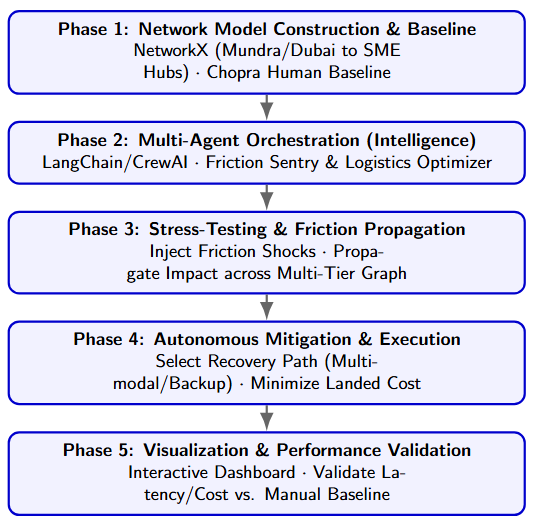
\includegraphics[width=0.65\textwidth]{Figures/methodology}
    \caption{Proposed methodology}
    \label{fig:methodology}
\end{figure}

\begin{itemize}
    \item \textbf{Phase 1: Network Model Construction \& Baseline Development:} Develop a multi-tier logistics graph using \texttt{NetworkX}, mapping critical nodes from international maritime chokepoints (e.g., Mundra, Dubai) to inland Indian SME clusters. Simultaneously, establish a Manual Human Planner baseline using Chopra inventory formulas to provide a performance benchmark for traditional, reactive supply chain management.
    \item \textbf{Phase 2: Multi-Agent Orchestration (Intelligence Layer):} Design and deploy specialized autonomous agents using \texttt{LangChain} and \texttt{CrewAI}. This includes a Friction Sentry for real-time monitoring of maritime signals (e.g., verification delays, insurance spikes, or congestion) and a Logistics Optimizer for executing autonomous rerouting and dynamic buffer-stock calculations.
    \item \textbf{Phase 3: Stress-Testing \& Friction Propagation:} Inject 1 simulated Friction Shock---ranging from administrative bottlenecks to regional blockades---into the graph model. The agents will identify these disruption signals, propagate the impact across the multi-tier supply chain, and evaluate the mathematical trade-offs of various mitigation strategies.
    \item \textbf{Phase 4: Autonomous Mitigation \& Execution:} The agentic pipeline autonomously selects the most efficient recovery path, such as pivoting to multimodal transport or identifying backup suppliers, to minimize Total Landed Cost and operational downtime. This phase transitions the system from simple "Detection" to "Executable Action".
    \item \textbf{Phase 5: Visualization \& Performance Validation:} Integrate the agentic output into an interactive Dashboard for real-time decision support. Validate the framework's effectiveness by comparing its response latency and cost-efficiency against the previously established manual baseline, targeting a measurable reduction in stockouts and overstocking.
\end{itemize}

\section[Expected Outcomes]{\textbf{Expected Outcomes}}
The expected outcomes of this project include:
\begin{itemize}
\item A functional multi-agent system using LangChain and CrewAI that transitions from passive monitoring to autonomous execution of mitigation strategies.
\item A dynamic NetworkX-based supply chain model integrated with a Tableau dashboard for real-time "What-If" scenario simulations and risk propagation visualization.
\item A validated framework demonstrating reduced operational costs and stock-outs for Indian SMEs compared to traditional manual planning.
\end{itemize}

\section[Organization of the Report]{\textbf{Organization of the Report}}
The remainder of this report is organized as follows:

\begin{itemize}
    \item \textbf{Chapter 2 - Theory and Fundamentals:} Discusses the theoretical foundations of Multi-Agent Systems, the Chopra inventory model, and the graph-theoretic principles used in the Logistics Digital Twin.
    \item \textbf{Chapter 3 - System Design:} Details the architectural design, agent roles, and the integration of CrewAI with the NetworkX graph model.
    \item \textbf{Chapter 4 - High-Level Implementation:} Elaborates on the development environment, API integrations (Gemini-Flash), and the execution logic of the agentic mitigation pipeline.
    \item \textbf{Chapter 5 - Detailed Design:} Focuses on the internal functional design, interaction protocols, and specific data structures used within the modular digital twin framework.
    \item \textbf{Chapter 6 - System Implementation:} Documents the coding standards, module connectivity, and the end-to-end integration of the backend services with the interactive dashboard.
    \item \textbf{Chapter 7 - Software Testing:} Presents the verification of modules and system workflows through unit, integration, and performance benchmarking suites.
    \item \textbf{Chapter 8 - Results and Discussion:} Analyzes the system's performance metrics and validates the agentic optimization results against human benchmarks.
    \item \textbf{Chapter 9 - Conclusion and Future Scope:} Summarizes the project's contributions, identifies current limitations, and proposes a roadmap for future technical enhancements.
\end{itemize}

\section[Summary]{\textbf{Summary}}
This chapter introduced the project domain, problem area, objectives, and significance of the
proposed work. It discussed the background, literature review, research gaps, methodology,
and expected outcomes of the project. The chapter also provided an overview of the overall
structure of the report. The information presented in this chapter establishes the foundation
for the detailed technical discussions provided in the subsequent chapters.











\fi

%Chapter 2
\ifINT
\input{./Chapter2/chapter2-Activity}
\else
\input{./Chapter2/chapter2-Funda}
\fi

%Chapter 3
\ifINT
\input{./Chapter3/chapter3-Task}
\else
\input{./Chapter3/chapter3-design}
\fi

%Chapter 4
\ifINT
\input{./Chapter4/chapter4-Reflection}
\else
\input{./Chapter4/chapter4-implement}
\fi

%Chapter 5
\ifINT
\else
\input{./Chapter5/chapter5-result}
\fi

%Chapter 6
\ifINT
\else
\input{./Chapter6/chapter6-conclution}
\fi

%Chapter 7
\ifINT
\else
\input{./Chapter7/chapter7-results}
\fi

%Chapter 8
\ifINT
\else
\input{./Chapter8/chapter8-conclusion}
\fi

%Chapter 9
\ifINT
\else
\chapter[Conclusion]{Conclusion}
This chapter presents the overall conclusion of the proposed project. It summarizes the work
carried out, highlights the major achievements of the system, and discusses the extent to
which the project objectives were achieved.

\section[Conclusion]{Conclusion}
This project addressed the critical problem of supply chain volatility and the lack of automated resilience in small and medium enterprise (SME) logistics networks through the development of an Agentic Supply-Chain Digital Twin. The proposed solution integrates a directed-graph model with a multi-agent orchestration layer powered by CrewAI. The major functionalities implemented include real-time friction detection, in-memory lead time calculation, and autonomous agent-driven rerouting. The system achieved a significant response speedup of 11.95 hours compared to the human baseline, effectively meeting all project objectives and proving highly applicable for enhancing SME logistics resilience.

\section[Limitations]{Limitations}
This section discusses the limitations and constraints of the proposed system:
\begin{itemize}
    \item \textbf{Strategic Scope:} The current implementation serves as a strategic digital twin focusing on high-level decision support rather than real-time tactical tracking.
    \item \textbf{Single-Shock Catering:} The system is currently optimized to process and mitigate one primary shock event per simulation cycle.
    \item \textbf{Regional Constraints:} The topology and business rules are specifically tailored for the Indian SME context, limiting immediate generalizability to other markets.
\end{itemize}

\section[Future Enhancement]{Future Enhancement}
Proposed improvements and future extensions for the system include:
\begin{itemize}
    \item \textbf{Dataset Expansion:} Increasing the richness of the dataset to include comprehensive multi-modal transport lanes.
    \item \textbf{Global Focus:} Expanding the target node focus beyond Indian SMEs to support international logistics corridors.
    \item \textbf{Operational Scaling:} Transitioning the framework into a fully operational digital twin by integrating live IoT telemetry and ERP data streams.
\end{itemize}

\section[Summary]{Summary}
The project successfully demonstrated the viability of agentic frameworks in autonomous logistics optimization. By addressing core SME vulnerabilities, the system achieved its goals of latency and cost reduction. While currently subject to certain functional and regional limitations, the identified future enhancements provide a clear path toward a fully operational, global supply chain resilience platform.





\fi

\backmatter
\ifDrf
\else
\clearpage
\addcontentsline{toc}{chapter}{Bibliography}
\printbibliography%
\fi

%% Uncomment the following 2 commands to add Appendix chapters
\appendix
\chapter{Plagiarism report}
The plagiarism check for this project report was conducted using an approved antiplagiarism tool prior to submission. The report confirms that the content of this work
is original and within the acceptable similarity threshold stipulated by RV College of
Engineering.

{\centering
    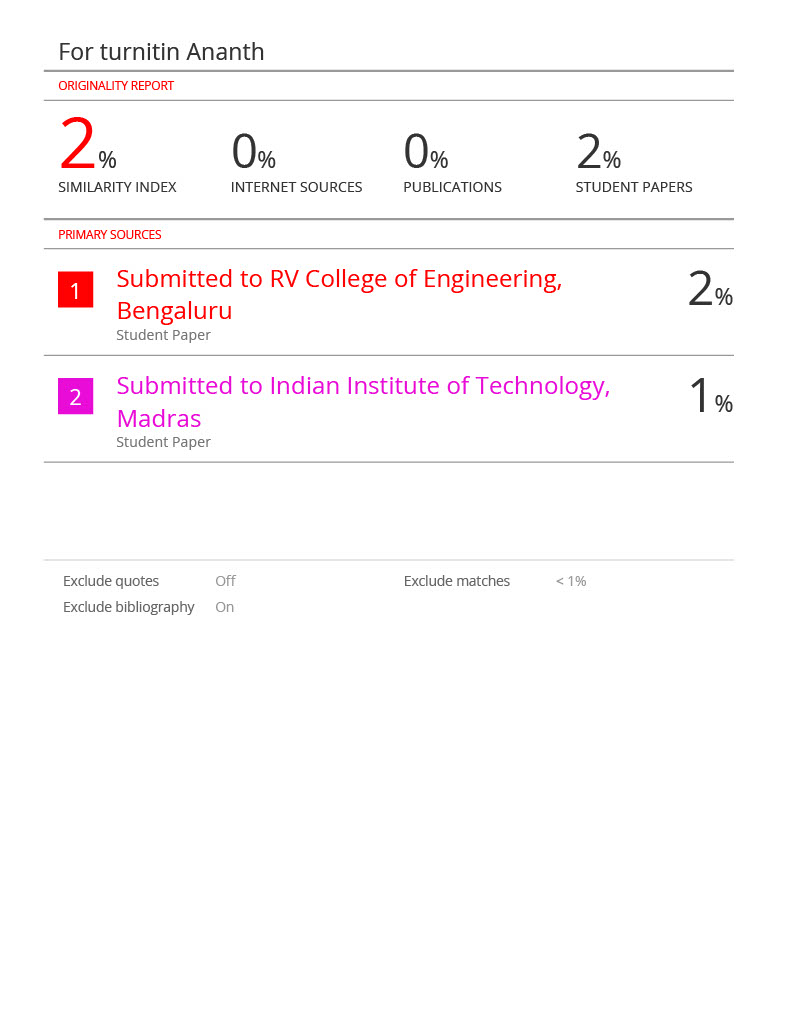
\includegraphics[width=0.95\textwidth,height=0.65\textheight,keepaspectratio]{Figures/Plagiarism report.jpg}
\par}
\clearpage

\chapter{Publication details}
The paper titled "Mitigating Logistics Friction in Global Chokepoints: An Agentic AI
Framework for Indian Export-Import Resilience" has been drafted. It will be submitted
for publication in a International Journal or Conference.

{\centering
    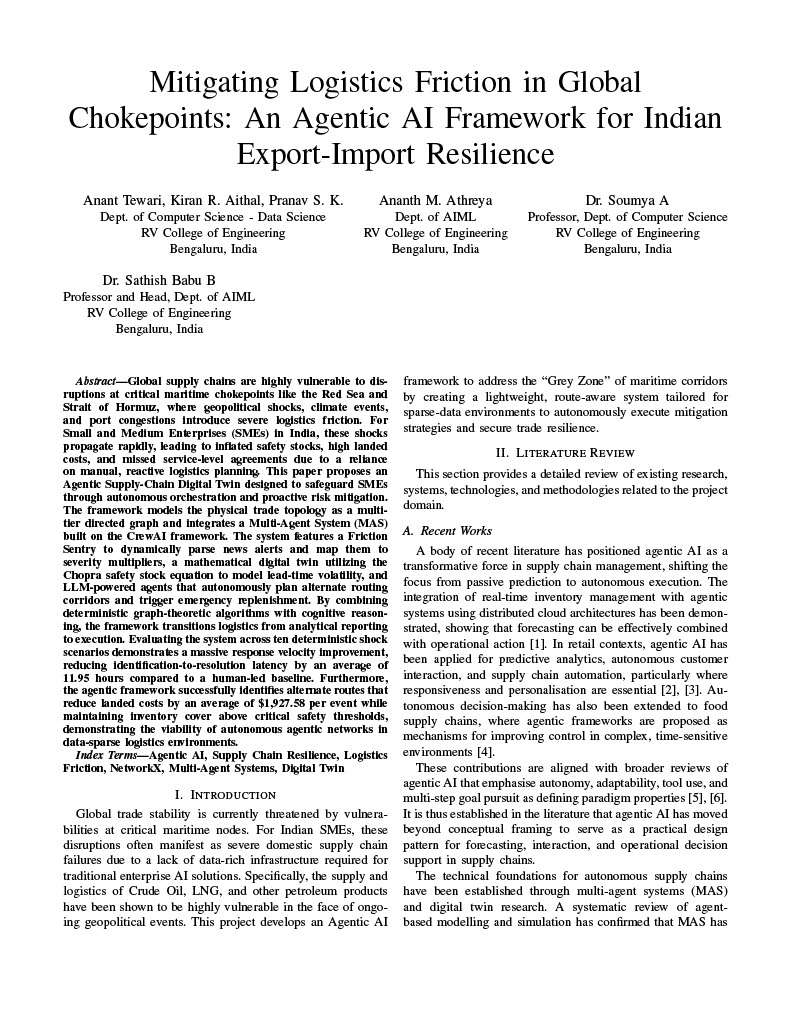
\includegraphics[width=0.95\textwidth,height=0.65\textheight,keepaspectratio]{Figures/P1.jpg}
\par}
\clearpage

\end{document}
